\documentclass[12pt]{article}
\usepackage{graphicx}
\usepackage{listings}
\usepackage[list=true,listformat=simple]{subcaption}
\usepackage{blindtext}



\begin{document}



\tableofcontents
\listoftables
\listoffigures
\lstlistoflistings



% --------------------------------------------------------------------
\newpage
\section{Introduction}



\blindtext


\begin{table}[ht]
\centering
    \begin{tabular}{c | c | c}
        Ord. & Name & Age \\
        \hline
        1 & John Smith & 20 \\
        2 & Talor Brown & 19
    \end{tabular}
\caption{Student list in my class}
\label{tab:student_list_in_my_class}
\end{table}


\blindtext


\begin{figure}[ht]
    \centering
    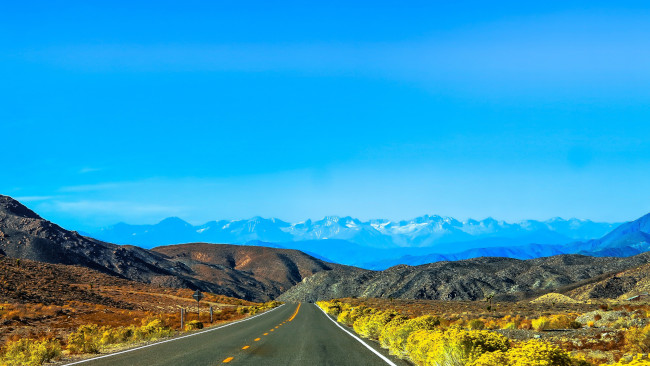
\includegraphics[width=8cm]{img/nextvoyage-road-moutain.jpg}
    \caption{Road Heading Towards Mountain by Nextvoyage}
    \label{fig:purple flower}
\end{figure}


\Blindtext[2]



% --------------------------------------------------------------------
\section{The Methods}



\subsection{Brief}



\blindtext


% captionpos=b ==> Insert the caption below the source code section
\begin{lstlisting}[language=Python, caption={Nested for loop in Python}, captionpos=b]
for i in range(5):
    for j in range(2):
        # Print a string
        print(f'i={i}, j={j}')
\end{lstlisting}


Maecenas pharetra convallis posuere morbi leo urna.
Laoreet non curabitur gravida arcu ac tortor dignissim.


\subsection{Steps}



Faucibus nisl tincidunt eget nullam non.
Arcu ac tortor dignissim convallis aenean et.


\begin{figure}[ht]
    \centering
    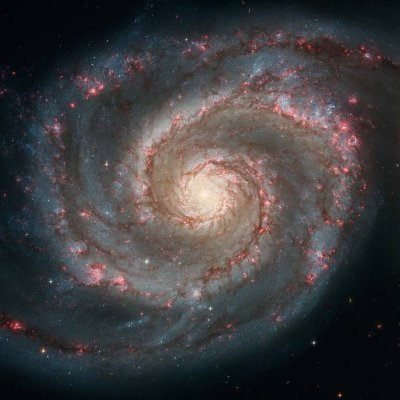
\includegraphics[width=6cm]{img/universe.jpg}
    \caption{The Universe}
    \label{fig:universe}
\end{figure}


\Blindtext[2]


\lstinputlisting[language=c++, caption={Point structure in C++}]{data/src_code_point.cpp}


Maecenas pharetra convallis posuere morbi leo urna.
Laoreet non curabitur gravida arcu ac tortor dignissim.



\subsection{Final result}



\blindtext


\begin{table}[ht]
\centering
    \begin{tabular}{c | c | c}
        Name & Strengths & Weaknesses \\
        \hline
        Old but Gold & Popular & Lack of features \\
        New and Fresh & Whole new architecture & Lack of community supports
    \end{tabular}
\caption{Strengths and Weaknesses of Methods}
\label{tab:method summary}
\end{table}


\blindtext



% --------------------------------------------------------------------
\section{Conclusion}



\blindtext


\begin{figure}[ht]
    \centering
    \begin{subfigure}{0.4\textwidth}
        \centering
        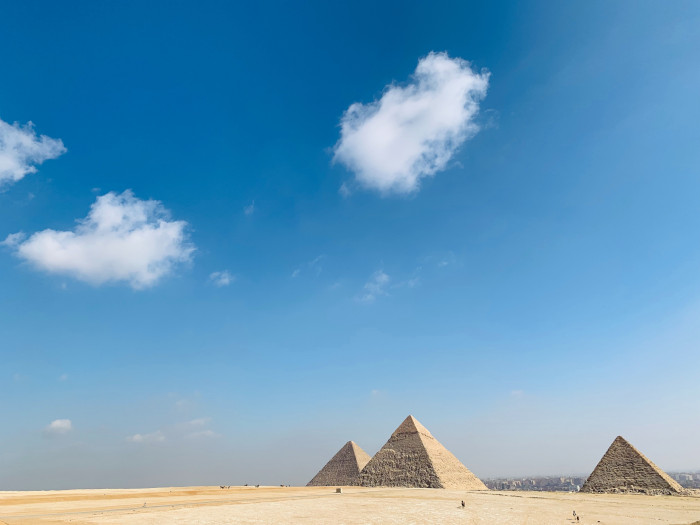
\includegraphics[width=\textwidth]{img/dave-ang-pyramid.jpg}
        \caption{Three Great Pyramid Under The Blue Sky by Dave Ang}
        \label{fig:great_pyramid}
    \end{subfigure}
    \hfill
    \begin{subfigure}{0.4\textwidth}
        \centering
        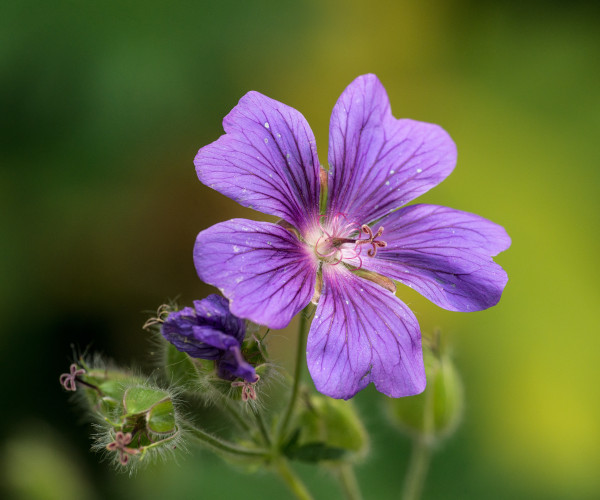
\includegraphics[width=\textwidth]{img/ganajp-purple-flower.jpg}
        \caption{Purple Flower by Petr Ganaj}
        \label{fig:purple_flower}
    \end{subfigure}
    \caption{Two Great Images}
    \label{fig:two_great_images}
\end{figure}


Diam vel quam elementum pulvinar etiam non quam lacus suspendisse.
Sed augue lacus viverra vitae congue eu.



\end{document}
